Przechodzimy teraz do etapu przygotowywania grafiki interfejsu gracza. W tej fazie skupiamy się na opracowywaniu elementów wizualnych, które będą bezpośrednio wpływały na doświadczenie użytkownika podczas interakcji z grą. Wykorzystujemy różnorodne narzędzia graficzne, aby stworzyć estetyczne, funkcjonalne elementy, obejmujące wszystko, od ikon po przyciski i panele.

Nasz cel to nie tylko stworzenie atrakcyjnego wizualnie interfejsu, ale także dostosowanie go do ergonomicznych potrzeb graczy, zapewniając czytelność, intuicyjność i efektywność w obszarze interakcji. Grafiki interfejsu gracza będą nie tylko ozdobą, ale przede wszystkim praktycznym narzędziem, które ułatwi użytkownikom korzystanie z różnych funkcji gry, podnosząc tym samym jakość ich doświadczenia.

\subsubsection{Przygotowanie listy grafik do stworzenia}

Przygotowywanie listy grafik do stworzenia to kluczowy krok w procesie projektowania. W tym etapie identyfikujemy i szczegółowo opisujemy wszelkie grafiki, które będą niezbędne do kompleksowego stworzenia wizualnej struktury projektu. Lista ta obejmuje różnorodne elementy, takie jak logo, ikony interfejsu, tła, animacje, czy też wszelkie inne grafiki, które są istotne dla spójnego wizualnego doświadczenia użytkownika.

W trakcie tworzenia tej listy uwzględniamy zarówno elementy dekoracyjne, jak i funkcjonalne, dbając o to, aby każdy element pełnił określoną rolę w kontekście użytkowego aspektu projektu. Sprecyzowane opisy pomagają zrozumieć, jakie oczekiwania mamy co do każdej grafiki, a także ułatwiają koordynację pracy zespołu, dając klarowny plan dla artystów grafików i projektantów.

\begin{center}
{\bfseries Lista grafik do stworzenia}
\end{center}
\begin{figure}[h]
    \centering
    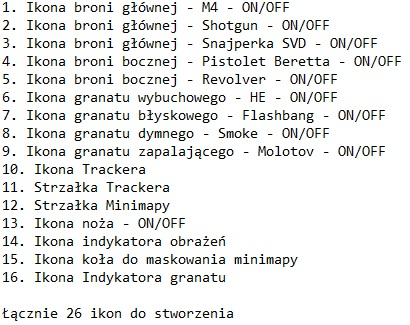
\includegraphics[scale=0.7]{Images/ListaIkon.jpg}
    \caption{Lista ikon do stworzenia}
    \label{fig:visBuglist}
\end{figure}
\FloatBarrier

\subsubsection{Poszczególne kroki tworzenia ikon}
Tutaj utworzymy ikonę, która będzie się wyświetlać podczas trzymania broni/granatu w ręku.
\begin{enumerate}
  \item Robimy screena prefabu wybranej broni. W tym przypadku Molotov.
\begin{figure}[h]
    \centering
    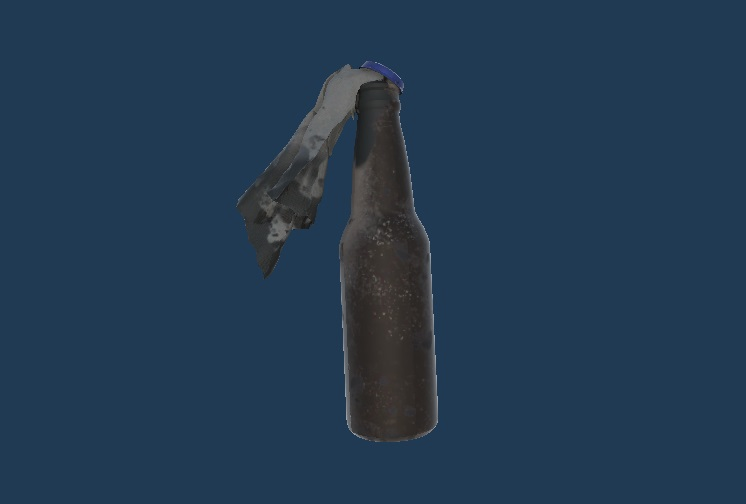
\includegraphics[scale=0.5]{Images/MolotovScreen.jpg}
    \caption{Screen prefabu}
    \label{fig:visBuglist}
\end{figure}
\FloatBarrier

  \item Wycinamy tło molotova, tak aby było przezroczyste.
\begin{figure}[h]
    \centering
    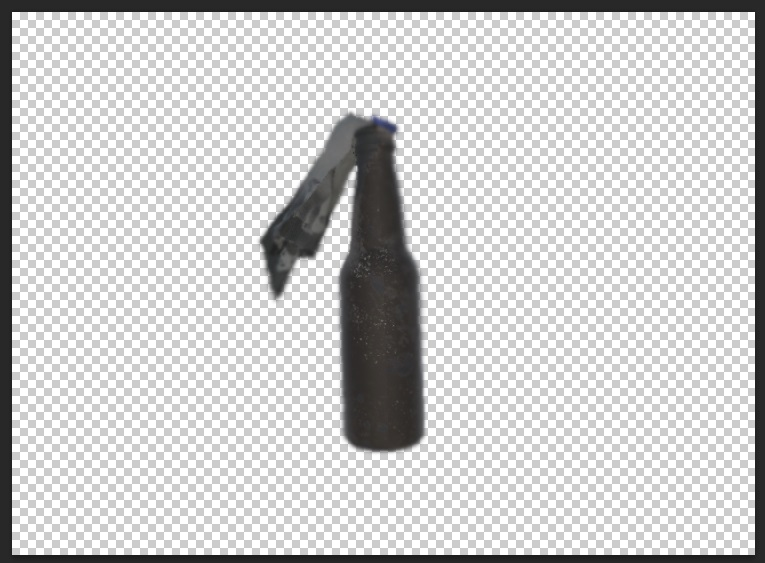
\includegraphics[scale=0.5]{Images/MolotovPNG.jpg}
    \caption{Usunięcie tła}
    \label{fig:visBuglist}
\end{figure}
\FloatBarrier

  \item Nakładamy na naszego Molotova biały kolor.
\begin{figure}[h]
    \centering
    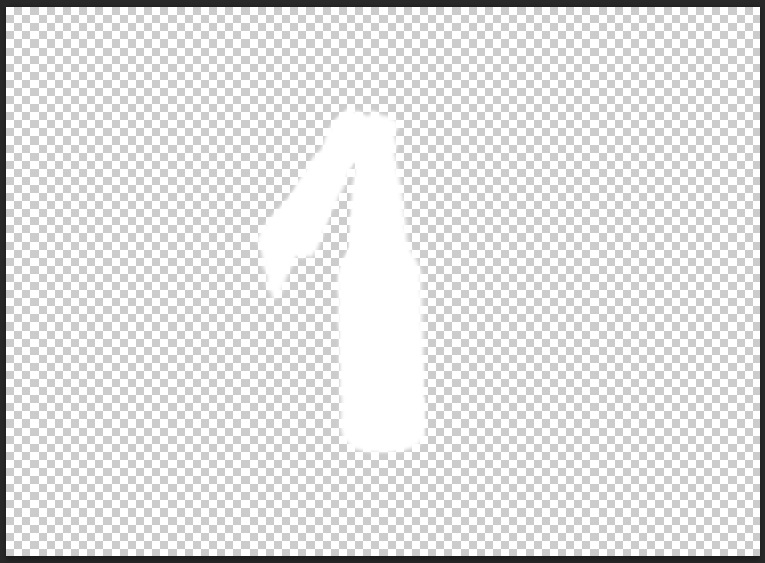
\includegraphics[scale=0.5]{Images/MolotovPNGWhite.jpg}
    \caption{Zmiana koloru na biały}
    \label{fig:visBuglist}
\end{figure}
\FloatBarrier

  \item W tym momencie nadajemy blask zewnętrzny grafice.
\begin{figure}[h]
    \centering
    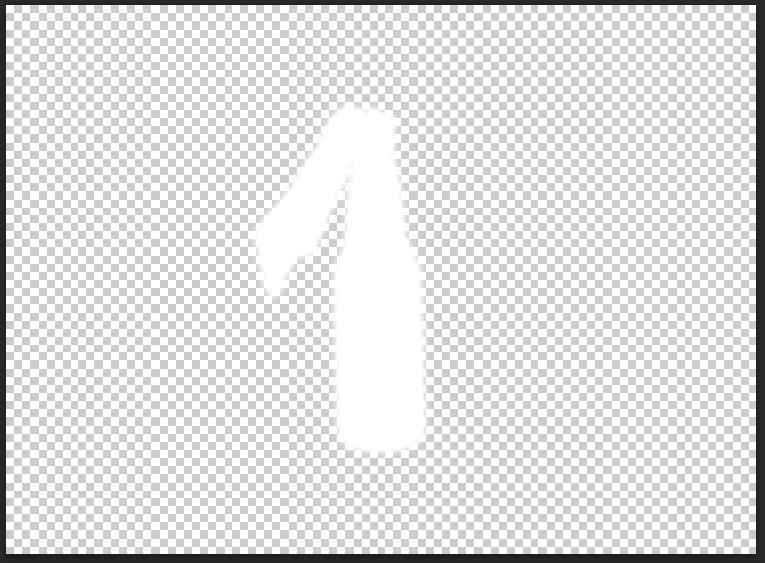
\includegraphics[scale=0.5]{Images/MolotovPNGWhiteBlask.jpg}
    \caption{Dodanie blasku zewnętrznego}
    \label{fig:visBuglist}
\end{figure}
\FloatBarrier

  \item Eksportujemy grafikę jako PNG.
\begin{figure}[h]
    \centering
    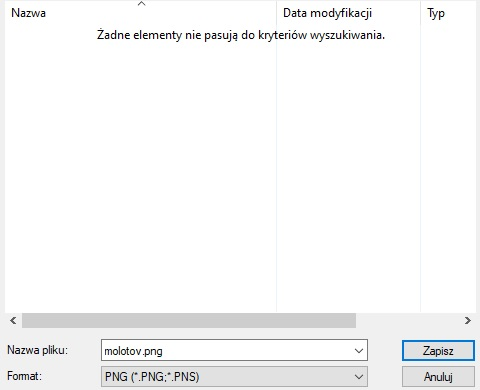
\includegraphics[scale=0.7]{Images/Saving.jpg}
    \caption{Eksport grafiki}
    \label{fig:visBuglist}
\end{figure}
\FloatBarrier
\end{enumerate}

Teraz utworzymy ikonę broni/granatu, która będzie się wyświetlała gdy posiadamy dany sprzęt bojowy w ekwipunku, ale nie trzymamy go w rękach. W tym przypadku powtarzamy \textbf{\textit{krok 1}} oraz \textbf{\textit{krok 2}}. Jeśli wykonamy poprzednie kroki możemy przystąpić do kolejnych.

\begin{enumerate}
  \item Nakładamy na naszego Molotova szary kolor.
\begin{figure}[h]
    \centering
    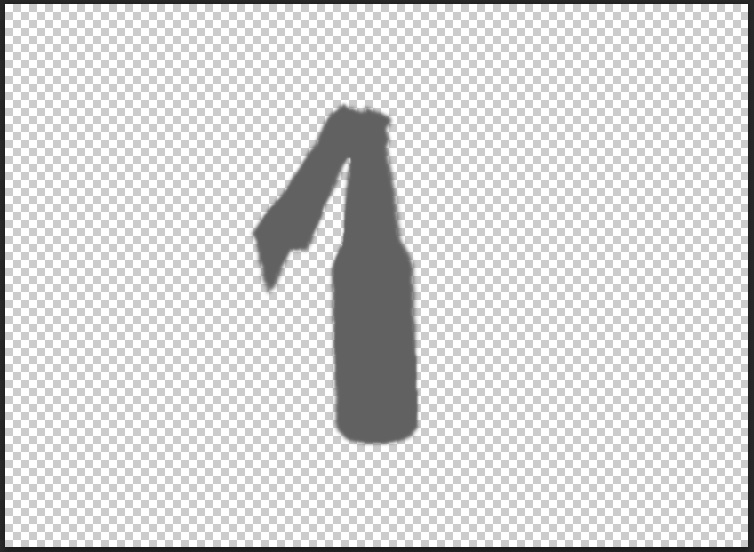
\includegraphics[scale=0.5]{Images/MolotovOFFgrey.jpg}
    \caption{Zmiana kolory na szary}
    \label{fig:visBuglist}
\end{figure}
\FloatBarrier

  \item Zmieniamy jego przezroczystość wedle upodobań.
\begin{figure}[h]
    \centering
    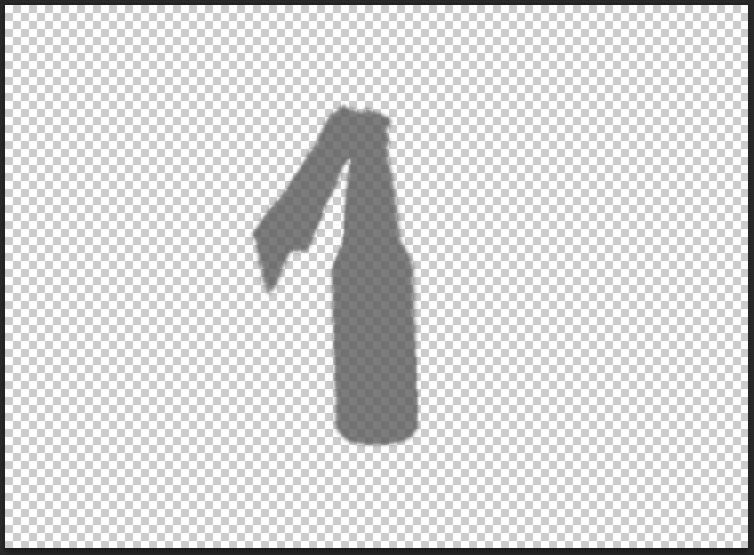
\includegraphics[scale=0.5]{Images/MolotovOFFgreyOpacity.jpg}
    \caption{Zmiana przezroczystości}
    \label{fig:visBuglist}
\end{figure}
\FloatBarrier
Jak możemy zauważyć nasze "przezroczyste" tło widać przez naszą ikonę, co oznacza, że nasza praca została wykonana pomyślnie.

  \item Eksportujemy grafikę jako PNG.
\begin{figure}[h]
    \centering
    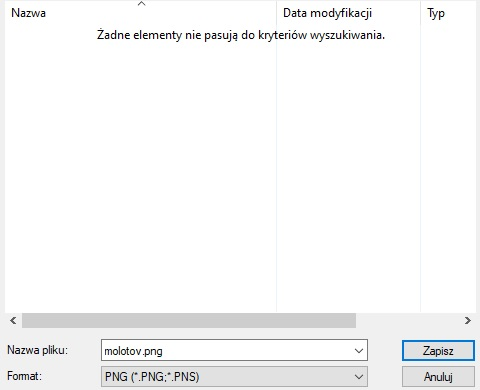
\includegraphics[scale=0.7]{Images/Saving.jpg}
    \caption{Eksport grafiki}
    \label{fig:visBuglist}
\end{figure}
\FloatBarrier
\end{enumerate}

Kolejnym krokiem jest powtórzenie tego samego procesu dla pozostałych ikon broni oraz granatów. W analogiczny sposób planujemy i tworzymy grafiki reprezentujące różne rodzaje broni oraz elementy wyposażenia, dbając o spójność wizualną z wcześniej opracowanymi elementami. Długość procesu oraz staranność w przygotowywaniu każdej ikony są kluczowe, aby zagwarantować zróżnicowanie i czytelność, jednocześnie zachowując estetyczny charakter całego zestawu. Ostatecznym celem jest stworzenie kompleksowego zestawu ikon, które będą jednoznacznie identyfikować różne elementy związane z uzbrojeniem w grze.

\subsubsection{Pokaz wszystkich granatów oraz broni zrobionych do gry}

\begin{figure}[h]
    \centering
    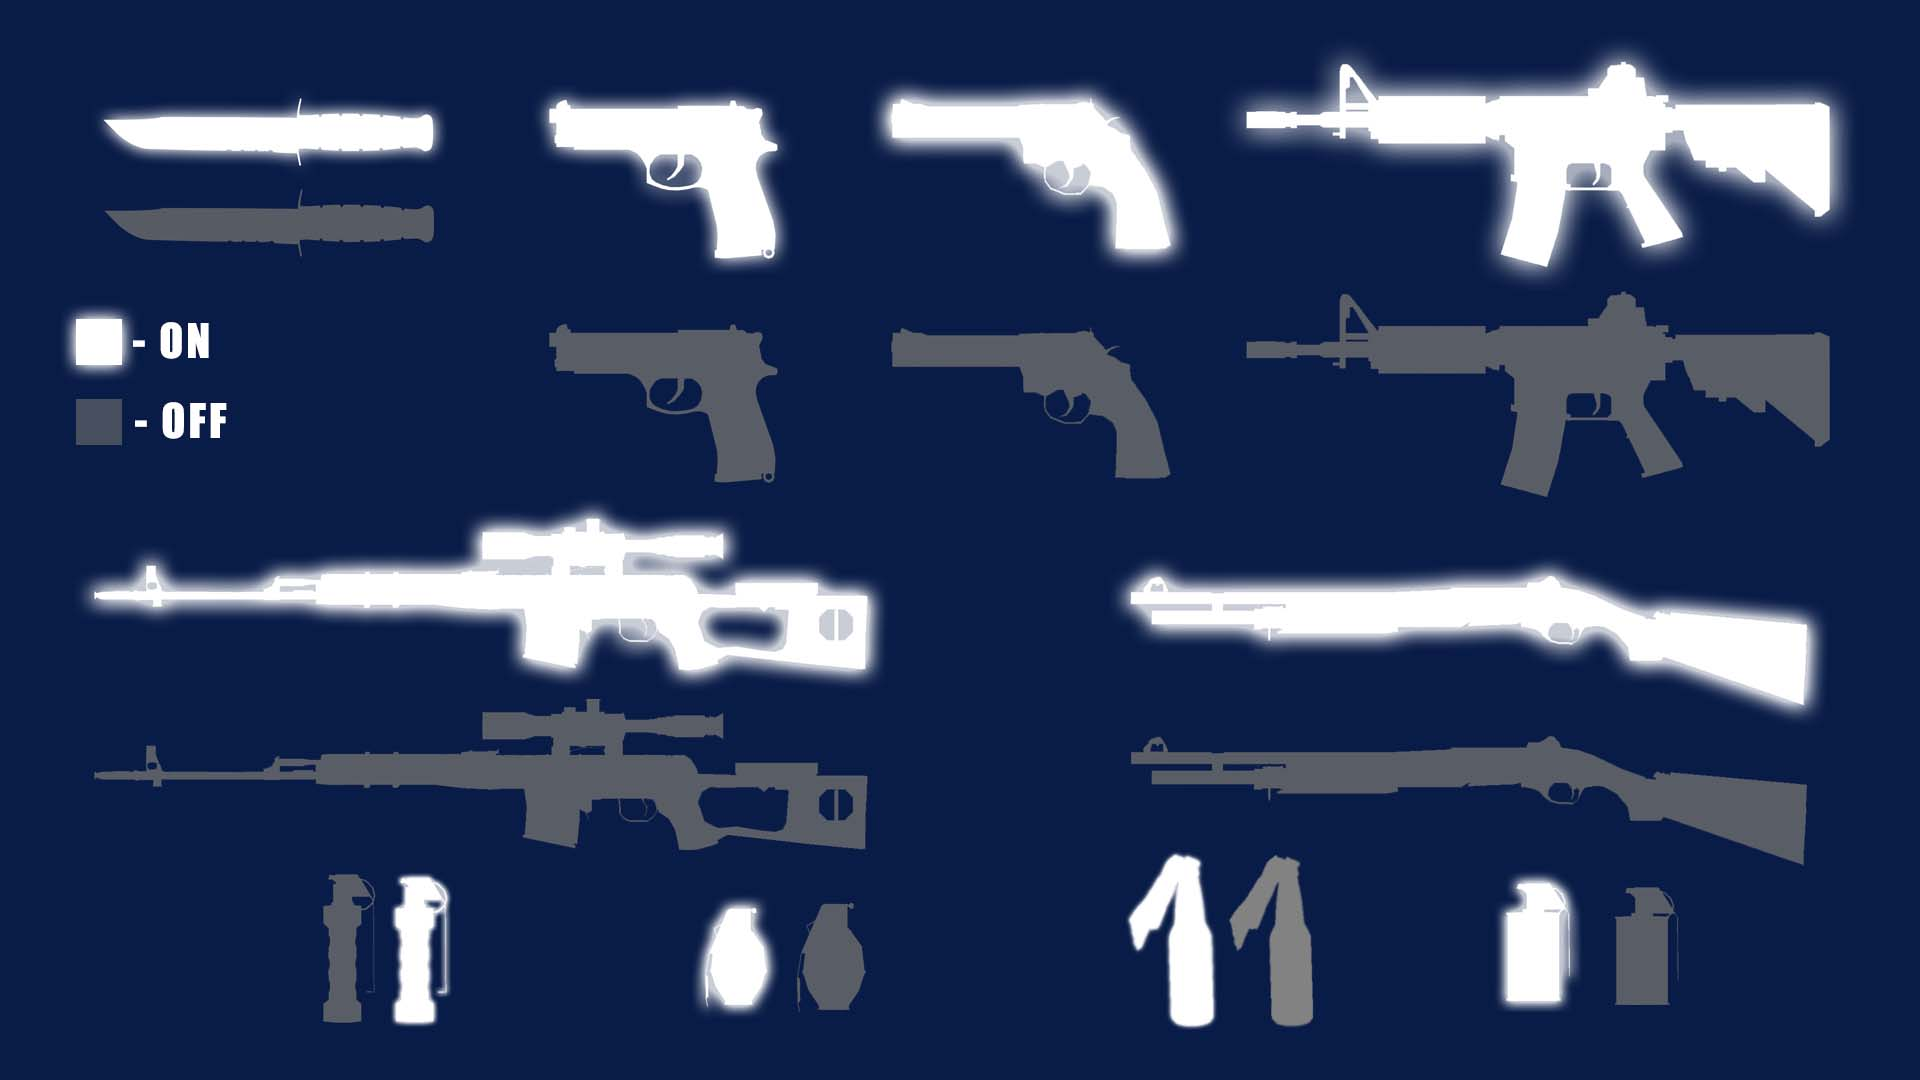
\includegraphics[scale=0.2]{Images/Pokazanie ikon broni.jpg}
    \caption{Plansza przedstawiająca wszystkie ikony broni oraz granatów w grze}
    \label{fig:visBuglist}
\end{figure}
\FloatBarrier

\subsubsection{Pokaz wszystkich ikon UI zrobionych do gry}

\begin{figure}[h]
    \centering
    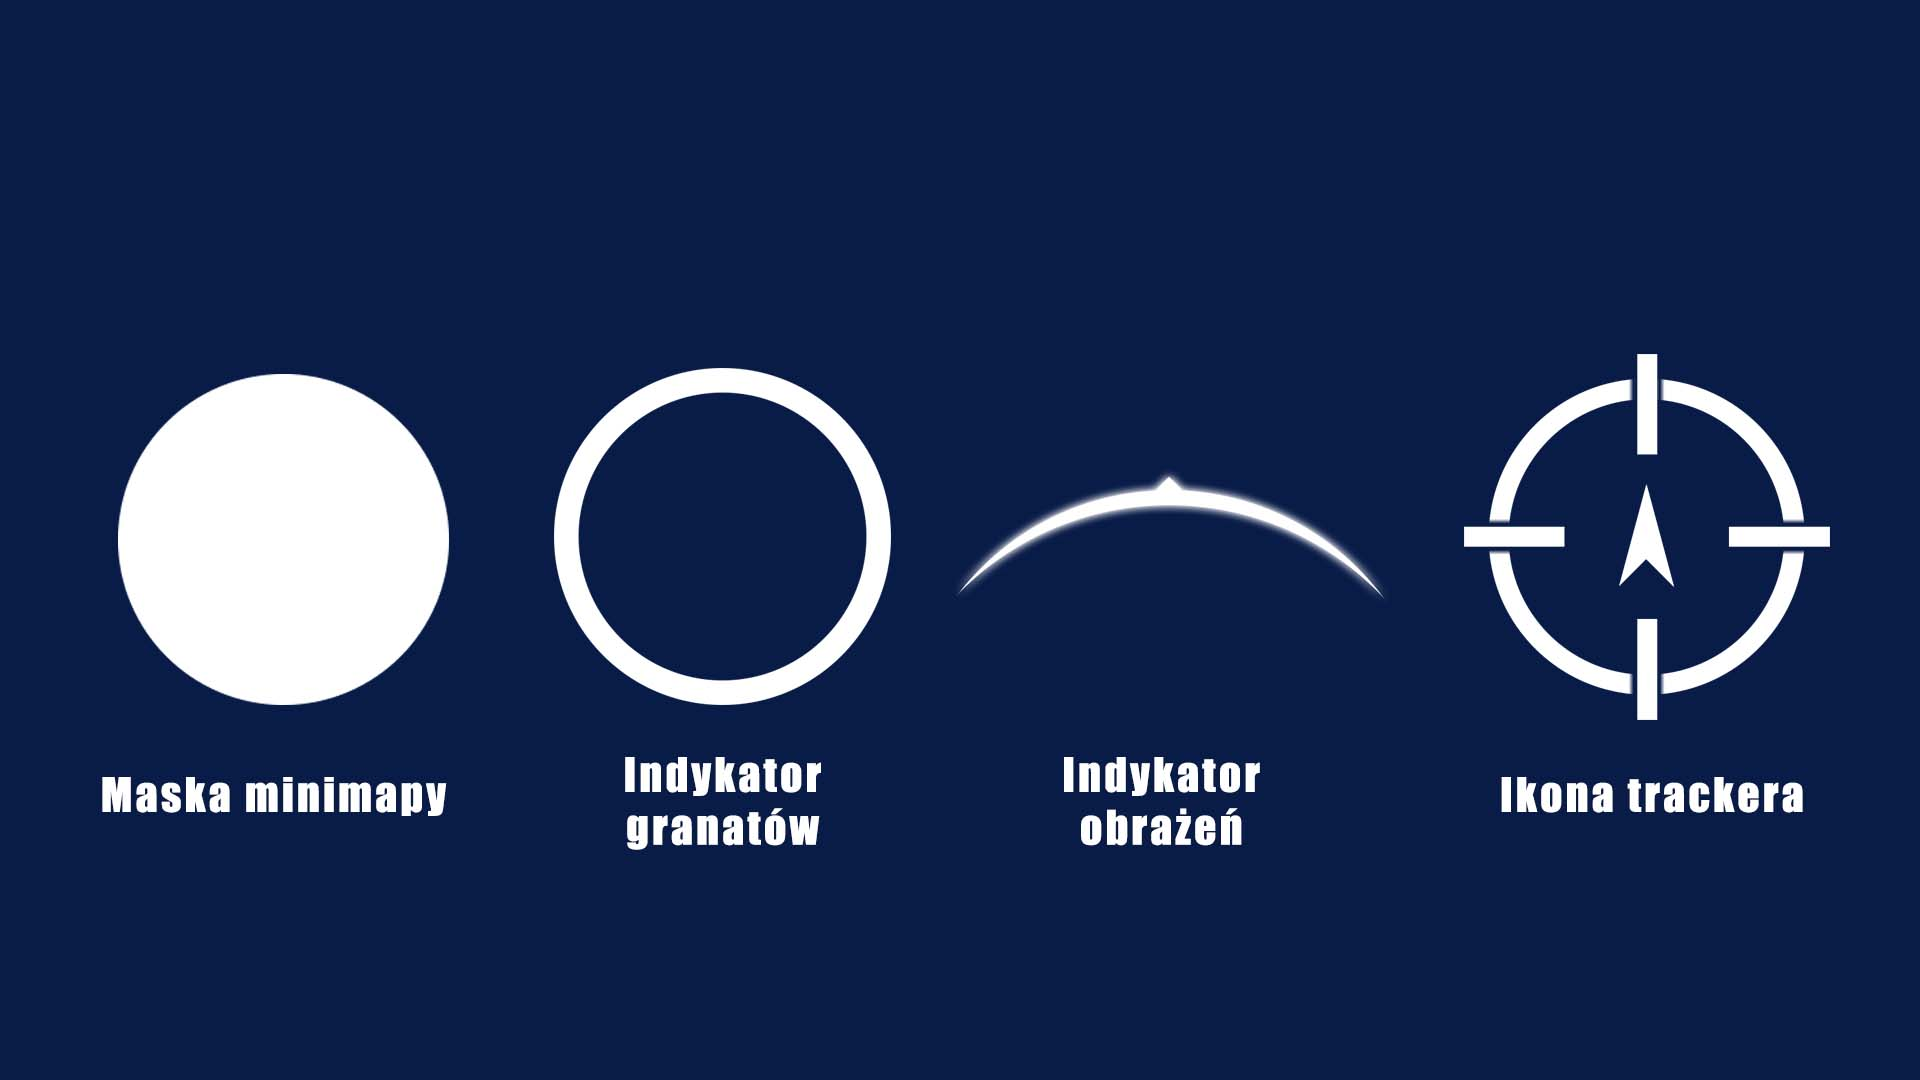
\includegraphics[scale=0.2]{Images/Pokazaniegranatow.jpg}
    \caption{Plansza przedstawiająca wszystkie ikony broni oraz granatów w grze}
    \label{fig:visBuglist}
\end{figure}
\newpage